\documentclass[class=book , crop=false]{standalone}

\usepackage{import} % Required for importing other .tex docs.  (import uses everything bw Begin and End Doc)
\usepackage{float} % Required for specifying the exact location of a figure or table
\usepackage{graphicx} % Required for including images
\usepackage{wrapfig}
\usepackage[pdftex,breaklinks,colorlinks=true,linkcolor=black,citecolor=blue,urlcolor=red,linktocpage=false,pagebackref=true,filecolor=magenta]{hyperref}%http://www.tug.org/applications/hyperref/manual.html#x1-100003.6
\usepackage{cite}
\usepackage[toc,title,page]{appendix}
\usepackage{pdfpages} % enables loading a pdf into the doc
\usepackage{makeidx}
\usepackage{glossaries} % must be after hyperref
\usepackage{blindtext}
\usepackage{enumitem}
%\usepackage{caption}

%\setlist[description]{leftmargin=\parindent,labelindent=\parindent}

%\renewcommand*{\bibname}{References} % renames the bibliography

\newcommand{\HRule}{\rule{\linewidth}{0.5mm}} % Command to make the lines in the title page

\graphicspath{{img/}{GIS_ChampionSection/img/}{awardsChapter/GIS_ChampionSection/img/}{brandPart/awardsChapter/GIS_ChampionSection/img/}{img/}{pairedProgSection/img/}{methodChapter/pairedProgSection/img/}{methodPart/methodChapter/pairedProgSection/img/}{documentationSection/img/}{methodChapter/documentationSection/img/}{methodPart/methodChapter/documentationSection/img/}{docStorageOrgSection/img/}{methodChapter/docStorageOrgSection/img/}{methodPart/methodChapter/docStorageOrgSection/img/}{QGisSection/img/}{toolsChapter/QGisSection/img/}{servicePart/toolsChapter/QGisSection/img/}{ESRISection/img/}{toolChapter/ESRISection/img/}{servicePart/toolChapter/ESRISection/img/}{../../../../source/}{../../source/}{servicePart/applicationsChapter/treasurerSection/img/}}

%\setlength\parindent{0pt} % eliminates indents


%\graphicspath{{img/}{GIS_ChampionSection/img/}{awardsChapter/GIS_ChampionSection/img/}{brandPart/awardsChapter/GIS_ChampionSection/img/}}

\title{ % create title page
\HRule % Horizontal Line added
\\[.4cm] % space
\begin{figure}[H] % included image
\begin{center}% centered horizontally
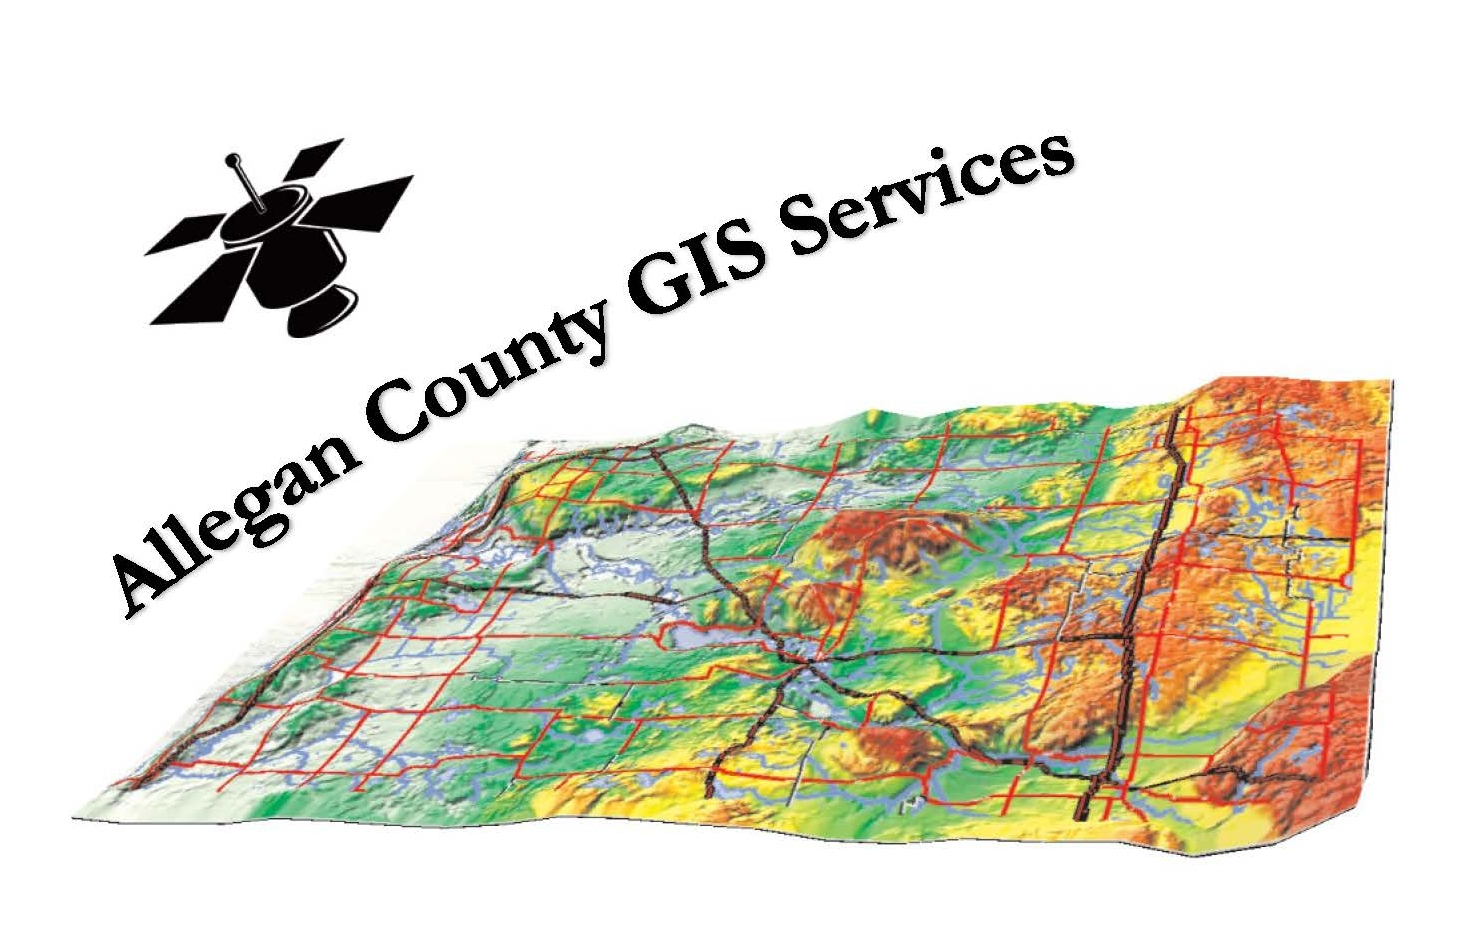
\includegraphics[scale=.45]{GIS_Logo_better.jpg}
\end{center}
\end{figure}
\Huge \bfseries GIS Champion Award Code % Title text
\HRule \\[.4cm] % Horizontal Line added
}  % closing brace for title

\author{\Large Allegan County GIS \\\Large www.allegancounty.org/gis} % defines author

%-------------------------------------------------------------------------
%Front Section %
%-------------------------------------------------------------------------
\begin{document} % Document Begins

% Comment / Uncomment this line to get the title when compiled here
%\maketitle % creates title page here when this page is compiled alone

\subsection{GIS Champion Award Code}

\begin{verbatim}

\documentclass[landscape]{article}
\usepackage{wallpaper}
\usepackage{niceframe}
\usepackage{xcolor}
\usepackage{ulem}
\usepackage{graphicx}
\usepackage{geometry}
\geometry{tmargin=.75cm,bmargin=.25cm,lmargin=.8cm,rmargin=.2cm}
\usepackage{multicol}
\setlength{\columnseprule}{0.4pt}
\columnwidth=0.3\textwidth

\begin{document}

%\TileWallPaper{4cm}{2cm}{CoLogo133x200.png}

\centering
\scalebox{3}{\color{green!30!black!60}
\begin{minipage}{.33\textwidth}
\font\border=umrandb
\generalframe
{\border \char113} % up left
{\border \char109} % up
{\border \char112} % up right
{\border \char108} % left
{\border \char110} % right
{\border \char114} % lower left
{\border \char111} % bottom
{\border \char115} % lower right
{\centering

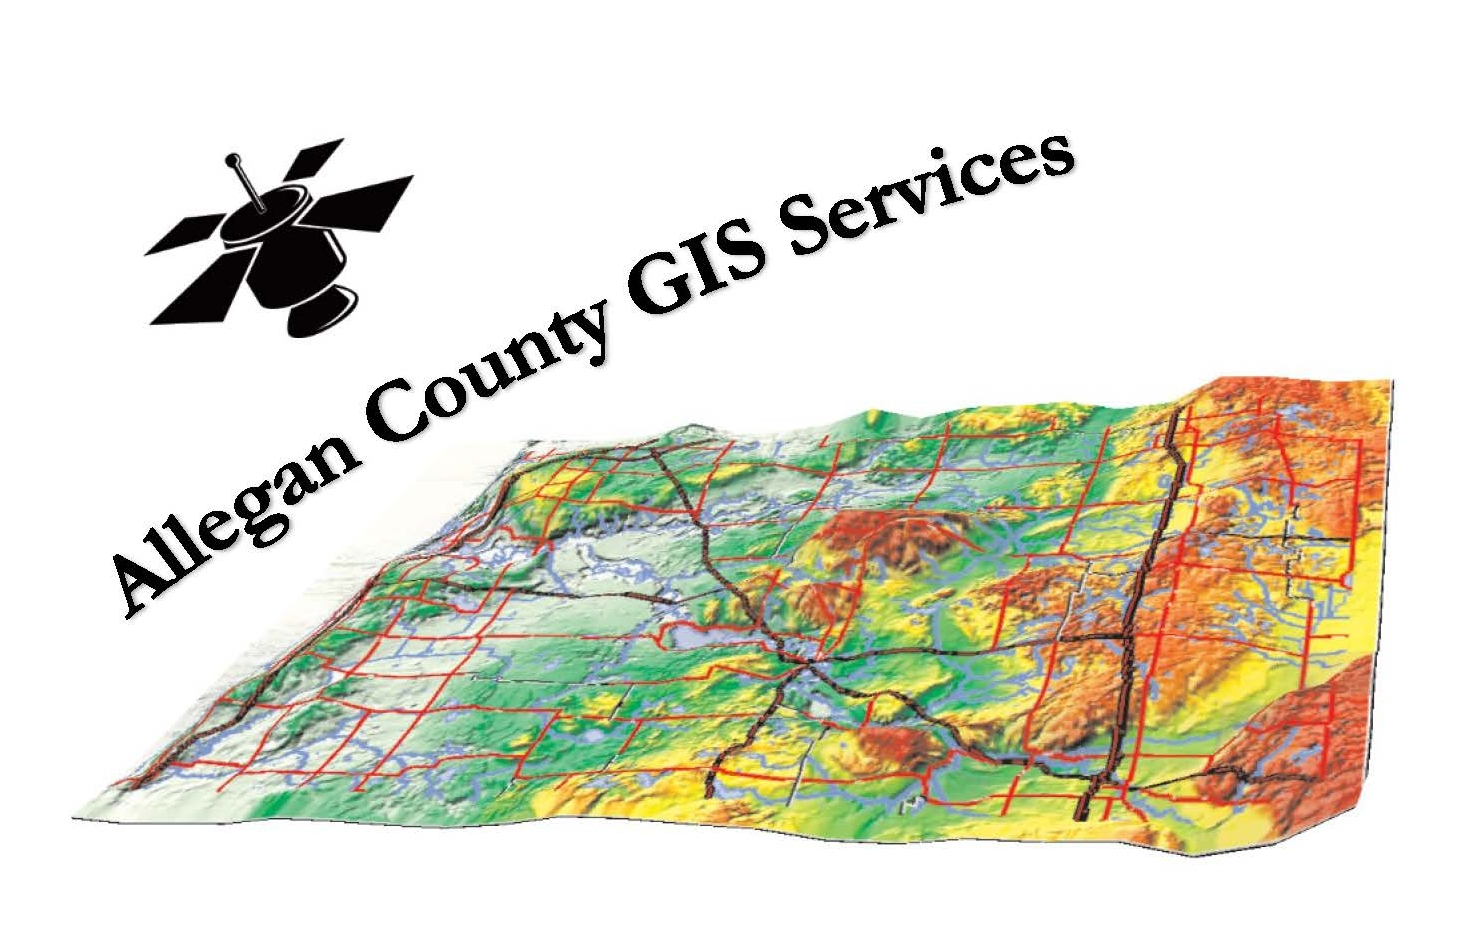
\includegraphics[height=1.25cm]{GIS_Logo_better.jpg}
%\end{minipage}
\vspace{-8mm}

\curlyframe[.9\columnwidth]{

\textcolor{red!10!black!90}
{\small Allegan County GIS Services}\\
\textcolor{green!10!black!90}{
\tiny recognizes}

\\
\uline{\textcolor{black}
{Ian Hanes}}
\\
\smallskip
\tiny Chief Equalization Technician
\smallskip

\textcolor{green!10!black!90}
{
\tiny as a
}
\smallskip
\tiny
\\
\textcolor{black}{\large \textsc{GIS Champion}}
\\
\vspace{1mm}
\textcolor{green!10!black!90}
{
\tiny for outstanding dedication and service to the community
\\while using GIS technology on this day
\itshape June 29, 2018
}
\vspace{3mm}

{\color{blue!40!black}
\scalebox{.6}{

\begin{tabular}{ccc}
\cline{1-1}
%\cline{2-2}
\cline{3-3}
%\cline{4-4}
%\cline{5-5}
\\
Neil Besteman  & &  Bryan May \\
GIS Manager & & GIS Analyst \\
\end{tabular}
}}}}
\end{minipage}

}
\end{document}


\end{verbatim}


\end{document}
